\documentclass[12pt,a4paper]{ctexart}
\usepackage{geometry}     % 設定邊界
\geometry{
  top=1in,
  inner=1in,
  outer=1in,
  bottom=1in,
  headheight=3ex,
  headsep=2ex
}
\usepackage[T1]{fontenc}
\usepackage{lmodern}
\usepackage{xeCJK}
\usepackage{amssymb,amsmath}
\usepackage{mathrsfs}
\usepackage{booktabs}
\usepackage{ifxetex,ifluatex}
\usepackage{indentfirst}
\def\tightlist{}
\usepackage{fixltx2e} % provides \textsubscript
% use upquote if available, for straight quotes in verbatim environments
\IfFileExists{upquote.sty}{\usepackage{upquote}}{}

% use microtype if available
\IfFileExists{microtype.sty}{\usepackage{microtype}}{}
\usepackage{graphicx}
% We will generate all images so they have a width \maxwidth. This means
% that they will get their normal width if they fit onto the page, but
% are scaled down if they would overflow the margins.
\makeatletter
\def\maxwidth{\ifdim\Gin@nat@width>\linewidth\linewidth
\else\Gin@nat@width\fi}
\makeatother
\let\Oldincludegraphics\includegraphics
\renewcommand{\includegraphics}[1]{\Oldincludegraphics[width=\maxwidth]{#1}}
\ifxetex
  \usepackage[setpagesize=false, % page size defined by xetex
              unicode=false, % unicode breaks when used with xetex
              xetex]{hyperref}
\else
  \usepackage[unicode=true]{hyperref}
\fi
\hypersetup{breaklinks=true,
            bookmarks=true,
            pdfauthor={陆思锐},
            pdftitle={液体粘度测量的三种方法},
            colorlinks=true,
            urlcolor=blue,
            linkcolor=magenta,
            pdfborder={0 0 0}}
\urlstyle{same}  % don't use monospace font for urls
%\setlength{\parindent}{0pt}
%\setlength{\parskip}{6pt plus 2pt minus 1pt}
\setlength{\emergencystretch}{3em}  % prevent overfull lines

%\usepackage{titling}
%\setlength{\droptitle}{-8em}  % 將標題移動至頁面的上面

\usepackage{fancyhdr}
\usepackage{lastpage}
\pagestyle{fancyplain}

\setcounter{secnumdepth}{5}

\title{液体粘度测量的三种方法}
\author{陆思锐\thanks{清华大学物理系\quad 基科52班 \quad 2015012206} }

\date{December 8, 2015}



\begin{document}

\maketitle



\begin{abstract}
粘度是流体的重要物理特性。粘度测量与石油、化工等工业技术的关系密切,生物、
医学等领域也常用到粘度测量。粘度分为动力粘度和运动粘度,一般将动力粘度简称为粘度。本实验通过旋转法、落球法、毛细管法来测量液体粘度并研究温度与液体粘度的关系。

\textbf{关键词:} 粘度,旋转,落球,毛细管
\end{abstract}



\tableofcontents
\section{实验目的}\label{ux5b9eux9a8cux76eeux7684}

\begin{itemize}
\tightlist
\item
  了解液体粘度测量的原理;
\item
  用旋转法测量液体的粘度、粘度与温度的关系曲线;
\item
  比较旋转法、落球法和毛细管法等测量液体粘度的方法。
\item
  研究温度与液体粘度的关系
\end{itemize}

\section{实验原理}\label{ux5b9eux9a8cux539fux7406}

\subsection{粘度的定义}\label{ux7c98ux5ea6ux7684ux5b9aux4e49}

粘度分为动力粘度和运动粘度,一般将动力粘度简称为粘度。

流体流动时流层间存在着速度差和运动逐层传递。当相邻流层间存在速度差时,快速流层力图加快慢速流层,而慢速流层则力图减慢快速流层。这种相互作用随着流层间速度差的增加而加剧。流体所具有的这种特性称为粘性,流层间的这种相互作用力称为内摩擦力或粘性(滞)力。粘度η是用来表示流体粘性程度的物理量,被定义为\(v_z=0\)的稳定层流中剪切应力\(\tau_{xz}=\frac{\Delta F}{\Delta S}\)
(F为切应力,S为表面积)与剪切速率\(\frac{d v_x}{d z}\)之比值。
\[\tau_{xz}=\frac{\Delta F}{\Delta S}=\eta\frac{d v_x}{d z}\]
动力粘度的单位是帕{[}斯卡{]}秒, 记作\(Pa\cdot s\)


实际工作中常常直接测量运动粘度\(v\),其定义为(动力)粘度\(\eta\)与流体密度\(\rho\)之比
\[v=\frac{\eta}{\rho}\] 运动粘度的单位是二次方米每秒, \(m^2/s\)

\subsection{用旋转法测定液体粘度}

实验中我们只讨论牛顿流体,即粘度\(\eta\)与\(\frac{d v_x}{d z}\)无关的液体。常见的水、轻质矿物油等较纯的流体都可以视为牛顿流体。

旋转法测量原理如图\ref{rotate},


\begin{figure}[htbp]
	\centering
	\begin{minipage}{0.4\linewidth}
	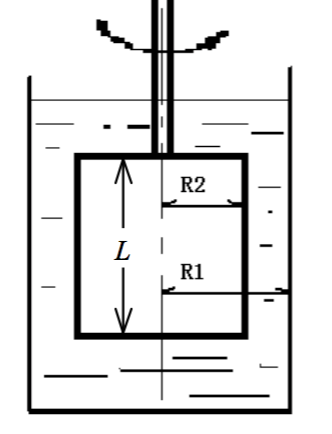
\includegraphics{media/14505376007114/rotate}
	\caption{旋转法装置图}
	\label{rotate}
	\end{minipage}
	\begin{minipage}{0.4\linewidth}
		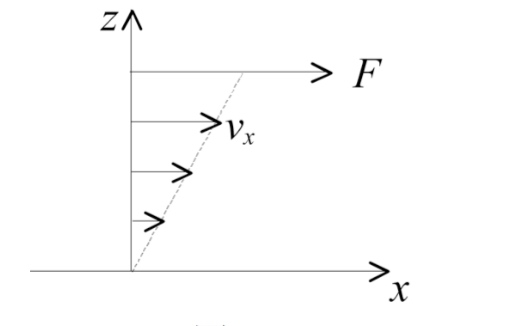
\includegraphics{media/14505376007114/14505392660186.jpg}
		\caption{原理示意图}
		\label{p}
	\end{minipage}
\end{figure}

当转子在液体中以稳定速度转动时,由牛顿内摩擦定律可知:面层流时流层间的内摩擦力等于表面积S、粘滞系数$\eta$和速度梯度\(\nabla v\)的乘积,即

\[F=\eta S\frac{dv}{d\mathbf{r}}\]

当液体产生稳定旋转时,对于如图4.2所示的高度为L的环状薄层,半径为r处的表面积\(S=2\pi rL\),该面所受的内摩擦力在柱坐标系中沿切线方向,其大小为

\[\mathbf{F_\phi}=\eta\mathbf{S}(-\mathbf{r}\frac{d \omega}{d\mathbf{r}})=-2\pi\eta\mathbf{Lr}(\mathbf{r}\frac{d \omega}{d r})\]

式中的负号是因角速度\(\omega\)沿径向递减之故。稳态旋转时半径为r的柱面所受的力矩为常数,设其值为M1,可得
\[M_1=rF_\phi=-2\pi\eta Lr^3\frac{d\omega}{d r}\]

利用边界条件\(\omega \mid_{r=R_2}=\omega_0\),\(\omega \mid_{r=R_1}=\omega_0\)可以得到

\[\omega_=\frac{M_1}{4\pi\eta L r^2}+c\]

再利用边界条件可以得到

\[\eta=\frac{M_1(R_1^2-R_2^2)}{4\pi LR_2^2R_1^2}\cdot\frac{M_1}{\omega_0}\]

此即Couette-Margules公式。

\subsubsection{液体粘度与温度的关系}

Andrade公式:
$$\eta=Ae^{E/kT}$$
T为绝对温度,k为玻尔兹曼常数,A、E为与液体分子结构有关的常数。测出样品液体二
个以上不同温度的\(\eta(T)\)值,即可定出E、A的值。E称为分子粘流活化能。如果E用克分子
活化能为单位,公式中k应乘以阿佛加德罗常数Na,kNa=R即摩尔气体常数。

\subsection{用落球法测定液体的粘度的原理}

当金属小圆球在粘性液体中下落时,它受到三个铅直方向的力:小球的重力\(\rho gV\)(V
是小球体积、\(\rho\)是小球密度)、液体作用于小球的浮力\(\rho_0gV\)(\(\rho_0\)是液体密度)和粘滞力f(其
方向与小球运动方向相反)。如果液体是无限深广的,而且小球的半径r和下落速度v均较小(Navior-Stokes方程的惯性项被忽略),则有
\begin{equation}
f = 6\pi\eta vr
\label{s}
\end{equation}

上式称为斯托克斯公式,其中$\eta$是液体的粘度,v是小球下落速度,r是小球的半径。

小球开始下落时,由于速度尚小,所以阻力也不大;但下落速度增大

\[\rho Vg=\rho_0 Vg+6\pi\eta vr\]

于是,小球作匀速直线运动。由上式可得:
\begin{equation}
\eta=\frac{(\rho-\rho_0)gV}{6\pi v}=\frac{2}{9}\frac{(\rho-\rho_0)gr^2}{v}
\label{eq46}
\end{equation}

如已知\(r、\rho、\rho_0\)和\(v\)等值,由测定匀速下落时的v值,即能计算\(\eta\)。实验时,待测液体必须盛于容器中(图\ref{luoqiu}),而小球
则沿筒的中心轴线下降,故不能满足无限深、广的条件,式\eqref{eq46}须作修改
\[\eta_0=\frac{2}{9}\frac{(\rho-\rho_0)gr^2}{v(1+2.4\frac{r}{R_0})(1+3.3\frac{r}{H})}=\frac{1}{18}\frac{(\rho-\rho_0)gd^2}{v(1+2.4\frac{d}{2R_0})(1+3.3\frac{d}{2H})}\]
其中$d=2r,R_0$为容器内半径,$H$为液柱高度。这是由于液体有边界,所测得的$v$较理想情况的为小,故须将式\eqref{eq46}等号右边项乘以小于1的因子,这样才能算得正确的\(\eta\)值。

\eqref{s}式(即斯托克斯公式)成立的条件:斯托克斯公式是由粘滞液体的普遍运动
方程导出的,要求小球的速度很小、球也很小,归结为雷诺数
\begin{equation}
R=\frac{dv\rho_0}{\eta}
\label{ll}
\end{equation}
很小。$R$很小的条件是因为在解方程时略去了一项有$R$因子的非线性项,如果考虑R,方程的解为
\[f = 6\pi\eta vr(1+\frac{3}{16}R-\frac{19}{1280}R^2+\cdots)\]
这叫做奥西恩-果尔斯公式。可以把由$(3/16)R$与\((19/1280)R^2\)项看作是斯托克斯公式
的一级修正项和二级修正项。如$R=0.1$时,则分别为,零级解与一级解相差约
\(2\%\),而二级修正项约\(2 \times 10^{-4}\)可不计;如 $R=0.5$,则零级解
与一级解相差约\(10\%\),二级修正项约\(0.5\%\)还可略去不计;当\(R≈1\)时,二级修正项约\(2\%\),
随着R的增大,高次修正项的影响变大,\eqref{s}式在R不太大的条件下才成立。不妨认为$Re\leq0.1$的时候成立。$Re\leq0.4$的时候用一级近似,有
\[f = 6\pi\eta vr(1+\frac{3}{16}R)\]
将\eqref{ll}式代入上式,再考虑\eqref{s}式的修正,可得
\[\eta_1=\frac{1}{36}\frac{(\rho-\rho_0)gd^2}{v(1+2.4\frac{d}{2R_0})(1+3.3\frac{d}{2H})}-\frac{3}{16}\rho_0dv=\eta_0-\frac{3}{16}\rho_0dv\]
$\eta_1$是1级修正后的结果,$\eta_0$是由\eqref{s}式算出的结果。 如果用二级修正,有
\[\eta_2=\frac{1}{2}\eta_1\left(1+\sqrt{1+\frac{19}{270}\left(\frac{\rho_0dv}{\eta_1}\right)}\right)\]

\begin{figure}[htbp]
\centering
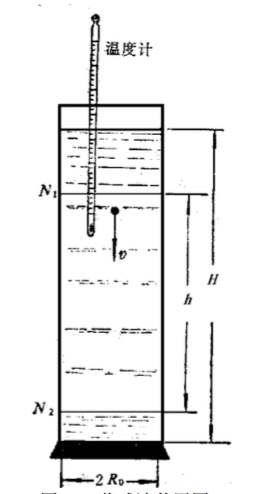
\includegraphics{media/14505376007114/14505414425530.jpg}
\caption{落球法装置图}
\label{luoqiu}
\end{figure}

长圆筒形玻璃容器如图\ref{luoqiu}所示,内盛待测液体,筒上约1/3与2/3处刻有两条刻度线
$N_1, N_2$,两线之间的距离为 h,实验时,当小球通过$N_1$时开始计时,到$N_2$时停止记时。
由此获得小球下落的速度$v=h/t$。筒的旁边挂有一支温度计,用以测量液体的温度,温度
计不要放入油中。另外还有两块磁铁,用以取出小球。

落球的挑选:用游标卡尺测量小球直径,令小球转到不
同的方向,测量其直径5-6次,如发现值相差很大,应舍去。

小球密度\(14.3×103 kg/m^3\),大球(d=2毫米)密度\(7.8×10^3kg/m^3\)。
注意:取小球要特别小心,不要丢失!注意油必须静止、小球要圆、表面要清洁,筒
要铅直,不要把油洒出筒外。

\subsection{用毛细管法测定液体的粘度}

毛细管粘度计,根据U型管的结 构,液体在重力作用下流动,测得
---定量液体流经上、下标线E、F 需要的时间,便可按照公式计算出
液体的运动粘度值。

\begin{figure}[htbp]
\centering
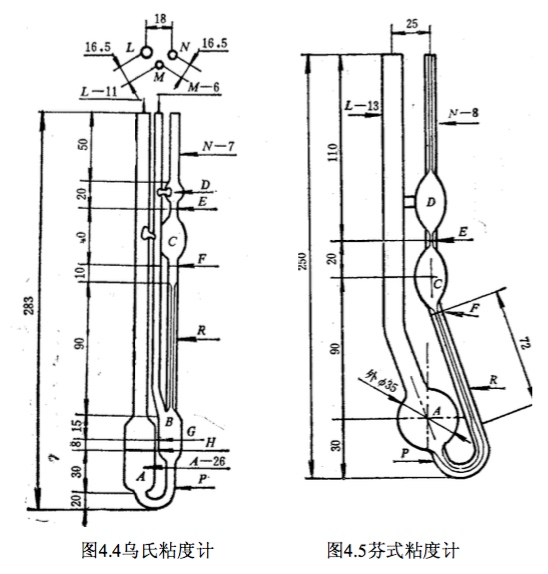
\includegraphics{media/14505376007114/14505415924880.jpg}
\caption{}
\end{figure}

关于液体的粘度有泊肃叶(Poiseuille)公式,即当液体在层流的情况下稳定地流过一均匀细管时,
\begin{equation}
d V={\frac {\pi r^{4}\Delta pdt}{8\eta L }}
\label{bsy}
\end{equation}


其中dV为dt时间内流过液体的体积;\(\Delta p\)为细管两端的压强差,r、l分别为细管的内半径和
长度,η为液体的粘度。由\ref{bsy}式可以求出\(\eta\),但是\(\Delta p,r,l\)等量难以测准,所以一般
用比较法测量η。由\ref{bsy}式得

\[\eta_2=\eta_1\frac{\rho_2t_2}{\rho_1 t_1}\]

由此可见,如果已知\(\eta_1\)则根据\(\rho_1、\rho_2\)测出$t_1,t_2$;就可以求得\(\eta_2\)。这样,我们只要用绝对测量法测准一种液体的粘滞系数,就可以相对地测定其他液体的粘滞系数,从而省去
了\(l,r,V,\Delta p\) 等量的测量.
用比较法测\(\eta\)时,需要保证在同一条伴下进行实验.同一个\(r,l\)是由仪器本身满足的;
同一个v要在测量时予以保证;还要保证粘滞器都维持铅直;在同一个温度下进行实验。

\section{实验仪器及注意事项}
\subsection{基本仪器}
\begin{enumerate}
	\item 旋转粘度计
	\item 恒温水浴箱
	\item 盛有蓖麻油的长圆筒型玻璃容器
	\item 直径维1mm和1.2mm的金属球
	\item 芬氏粘度计
	\item 游标卡尺
	\item 秒表
	\item 游标卡尺
\end{enumerate}
\subsection{注意事项}
\textbf{毛细管粘度计}的使用是否正确,与很多因素有关,如温度影响,装置震动的影响,检定用标准液、标准温度计、秒表等准确程度的影响,以及调节垂直度,记录时间,操作者主观因素等影响。

粘度计的清洗是粘度测定中十分重要的环节,粘度计内壁如不清洁,液体在里面流动将受到不应有的阻力或滑动,影响流出时间的正常测定.有时,同一个系列的粘度计重复测量液体的流动时间长短相差很大,造成重复性超差使整组测定数据无效.有时在一个系列里重复性没有超差,但进行平行测定时,两个系列数据超出允许误差范围,而必须重新清洗,重新进行测定。


本实验使用\textbf{乌氏粘度计}。乌氏粘度计适用于透明液体的测量,乌氏粘度计在U型结构上,毛细管的下端加一个悬挂水平球,悬挂水平球的左上方接一个管M,这一结构上的特点便形成了乌氏粘度计的优点,见图。


\section{实验步骤}\label{ux5b9eux9a8cux6b65ux9aa4}

\begin{itemize}

\item
  用\textbf{旋转法}测量蓖麻油在室温下至$60^{\circ}C$范围内的粘度变化,绘出粘温曲线并与公式比较。
  \item 不变换测定容器和转子(系数因子:10),用毕不用洗。
  \item $45^{\circ}$以下$\eta$变化快,采点间隔为$2\sim3^{\circ}C$,$45\sim60^{\circ}C$:采3点即可。
  
\item 用\textbf{落球法}测定液体的粘度:取小球测量其直径6次,然后将其放入盛有\textbf{蓖麻油}的长圆筒形玻璃容器中,待其通过第一根刻度时开始计时,经过第二根刻度时计时结束。测量量刻度间间距,玻璃筒内径,第二根刻度线与桶底的距离。
\item 1.2mm和1.0mm两种直径的小球各测一组,小球不需要取出。仅仅对(5.9.9)式结果计算$U_{\eta}$ 另外两个不计算U 不做油桶倾斜。选作小球偏离D/3

\textbf{毛细管法} (标准液为水,待测液为酒精)
\item 粘度计在测量前用自来水反复冲洗,最后用蒸馏水冲洗,吹干。
 然后用自来水将乌式粘度计冲净,用少量纯水冲洗两次,将纯水经L注入A中,液面达到m4和m3之间(约15ml),粘度计放在架子上,注意不要拧紧,以免夹碎粘度计,粘度计垂直放置。
 \item 给L管打气,当M管液面超过B泡时,堵住M管,当液面达到D泡一半时,停止打气,放开M管,当液面通过m1m2区间时计时,选取适当的粘度计,使其在粘度计内的流动时间不小于200 s(因条件限制,该实验只有一种粘度计,流动时间小于200s)。
\item 测酒精粘度:倒出纯水,用注射器抽取少量未知液体,注入粘度计,冲洗两次,以下与测量纯水相同。
  \item 数据处理
\end{itemize}

\section{实验数据}

\subsection{用旋转法测定液体的粘度}
k=10

% Table generated by Excel2LaTeX from sheet '旋转法'
\begin{table}[htbp]
  \centering
  \caption{旋转法实验数据}
    \begin{tabular}{rrrrrr}
    \toprule
    温度T($^{\circ}C$) & a     & $\eta$ & $\ln{\eta}$ & 1/T   &  \\
    \midrule
    26.0  & 59.0  & 0.590 & -0.5276327 & 0.003342805 &  \\
    28.0  & 55.0  & 0.550 & -0.597837 & 0.003320604 &  \\
    30.0  & 46.0  & 0.460 & -0.7765288 & 0.003298697 &  \\
    32.0  & 40.0  & 0.400 & -0.9162907 & 0.003277077 &  \\
    34.3  & 34.0  & 0.340 & -1.0788097 & 0.003252561 &  \\
    35.9  & 30.0  & 0.300 & -1.2039728 & 0.003235722 &  \\
    36.4  & 29.0  & 0.290 & -1.2378744 & 0.003230496 &  \\
    37.5  & 25.0  & 0.250 & -1.3862944 & 0.003219057 &  \\
    38.5  & 23.5  & 0.235 & -1.4481698 & 0.003208728 &  \\
    39.0  & 22.0  & 0.220 & -1.5141277 & 0.003203588 &  \\
    40.0  & 20.0  & 0.200 & -1.6094379 & 0.003193358 &  \\
    41.0  & 19.0  & 0.190 & -1.6607312 & 0.003183193 &  \\
    42.0  & 18.0  & 0.180 & -1.7147984 & 0.003173092 &  \\
    43.0  & 17.0  & 0.170 & -1.7719568 & 0.003163056 &  \\
    44.0  & 16.0  & 0.160 & -1.8325815 & 0.003153082 &  \\
    45.0  & 15.0  & 0.150 & -1.89712 & 0.003143171 &  \\
    50.0  & 11.0  & 0.110 & -2.2072749 & 0.003094538 &  \\
    55.0  & 9.0   & 0.090 & -2.4079456 & 0.003047387 &  \\
    60.0  & 7.0   & 0.070 & -2.65926 & 0.003001651 &  \\
    B     & 6605.38681 & $s_B$ & 172.936022 & $U_B$ & 360.7382211 \\
    $\ln{A}$截距 & -22.614323 & $s_{\ln A}$ & 0.55306176 & $U_{\ln A}$ & 1.153666624 \\
    A     & 1.5091E-10 &       &       & $U_A$ & 1.74102E-10 \\
    理论计算值   & 0.70629405 &       &       &       &  \\
    蓖麻油粘度 & 0.7559195 &       &       &       &  \\
    \bottomrule
    \end{tabular}%
  \label{tab:addlabel}%
\end{table}%
可见理论值和测得值有一定差距,这可能是因为温度不准。具体分析在讨论中。


\subsection{用落球法测定液体的粘度}
$$\eta=\frac{1}{18}\frac{(\rho-\rho_0)gd^2}{v}$$

% Table generated by Excel2LaTeX from sheet '落球法'
\begin{table}[htbp]
  \centering
  \caption{落球法数据}
    \begin{tabular}{|r|r|r|r|}
    \toprule
          & 小球直径d/m & 室温T   &  t/s \\
          \midrule
    1     & 0.001200 & 23.5  & 40.37 \\
    2     & 0.001185 & D/m   & $U_D$ \\
    3     & 0.001185 & 0.05890 & 0.00002 \\
    4     & 0.001180 & h/m   & $U_h/m$ \\
    5     & 0.001195 & 0.2350 & 0.0005 \\
    6     & 0.001205 & H/m   & $U_H/m$ \\
    7     & 0.001200 & 0.1200 & 0.0005 \\
    8     & 0.001190 & $\rho_0(kg/m^3)$ & $U_{\rho}(kg/m^3)$ \\
    d     & 0.001193 & 959.571 & 5.E+01 \\
    标准差   & 8.86E-06 & $\rho(kg/m^3)$ &  \\
    相对标准差 & 0.74\% & 7.80E+03 &  \\
    A类不确定度 & 8.2E-06 & 粘度(未修正) & 9.10E-01 \\
    B类不确定度 & 0.000004 & 雷诺数   & 5.95E-02 \\
    不确定度  & 9.12E-06 & 奥森近似  & 9.20E-01 \\
    相对不确定度 & 0.76\% & 最终修正  & 8.65E-01 \\
    结果    & $0.0011193\pm 0.000009 $&       &  \\
    \bottomrule
    \end{tabular}%
  \label{tab:addlabel}%
\end{table}%

只计算未修正的时候的不确定度

$$U_{\eta}=\eta\sqrt{\left(\frac{U_{\rho_0}}{\rho_0-\rho}\right)^2+4\left(\frac{U_d}{d}\right)^2+\left(\frac{U_h}{h}\right)^2+\left(\frac{U_t}{t}\right)^2}=0.013$$
相对不确定度为1.43\%
最终得到
$$\eta=0.91\pm0.01 Pa\cdot s$$
\subsection{用毛细管法测定液体的粘度}
酒精和水都取用14ml
$$\nu=\frac{\eta}{\rho}=\frac{\nu_w}{t_w}t=(\frac{\eta_w}{\rho_wt_w})t$$


查表可得水在$22^{\circ}$时为$997.8003kg/m^3$,$25^{\circ}$时为$997.0751kg/m^3$。实验室室温为$23.5^{\circ}$,不妨取两者的平均值为$997.4377kg/m^3$

根据\cite{jcwlsyjy}纯水的粘度有经验公式

$$\eta_{H_2O}=4.040625\times 10^{-2}\exp{\frac{418.6322}{t+110.4}}$$

代入可得到水的粘度为0.921mPa

测得$t_{water}=t_w=147.73s 
)$,$t=247.32s
)$(已经换成了10进制)
那么可算得

$$\nu=0.00155 Pa\cdot s$$

似乎和文献中的标准值有一定差距,这可能是因为酒精纯度不够(粘度计里面有水或者酒精本身纯度就不够)。

\section{实验讨论}
\subsection{旋转法}
\begin{enumerate}
\item 等待时间不够久的话温度不会稳定,恒温水浴仪的温度可能会与设定的温度不同。有可能高也有可能低。
\item 应该读取粘度计的温度而不是水浴仪的温度。可以通过观察粘度指针是否晃动来判断是否稳定了。
\item 要适当安置好粘度计的转子使其浸没在液体中、两轴线要重合,尽量使之没用晃动。
\item 有一个关于数据处理的疑问。由不确定度公式有$\frac{U_A}{A}=U_{lnA}$,当$\ln{A}$很大的时候,相对不确定度可以非常轻易地超过1。
\end{enumerate}
\subsection{落球法}
\begin{enumerate}
	\item 实验中皮筋要碎片,读数的时候视线要和皮筋平面平齐。避免视差
	\item 公式成立的条件是小球已经达到匀速。用简单的近似估算可以得出,小球加速距离很短。文献\cite{张兆钧1995用落球法测量η实验中小球下落速度的辨析},\cite{王丽娟2009探究落球法测液体黏度实验中小球达匀速运动所需的时间}
	\item 当小球偏离轴线时,受到的阻力会变大。时间变长,文献\cite{李向亭2009落球法测量粘滞系数中的边界问题——水立方的魔力之谜}得出时间和偏离距离经验上成二次函数关系。导致粘度系数偏大,当偏离$D/3$时误差为$0.3\%$左右。
	\item 我们发现测量值比旋转法和理论计算的都大,这可能是因为蓖麻油容易挥发,也可能是因为温度计测量的室温不是蓖麻油的温度,而蓖麻油对温度比较敏感。
	\item 本来是应该把球用磁铁吸出来重复实验的,但是油底球太多了所以只能放弃。
\end{enumerate}
\subsection{毛细管法}
\begin{enumerate}
	
	\item 这个实验很难评定不确定度,所以就不评定了。
	\item 由于时间较长且多次测量误差比较小,可以只测一组数据。
	\item 可以使用洗耳球将液体从一边吹回初始状态,不需要重新配置即可再次测量,多次测量可以提高精度。
	\item 通过查资料,发现实验数据有一定出入,可能是因为酒精不纯造成的。
\end{enumerate}
\section{致谢}

感谢物理52刘良洋同学,我们对某些问题进行了有益的讨论。

\bibliographystyle{plain}
\nocite{jcwlsyjy,jcwlsyjc}
\bibliography{ref}

\end{document}